\documentclass[a4paper,twocolumn]{article}
\usepackage[hmargin={1.1cm,1.1cm},vmargin={2.2cm,2cm}]{geometry}
%       includehead,     scale=0.85,centering,hoffset=-0.1cm,voffset=-0.5cm]{geometry} headheight=13.1pt ,portrait

%\usepackage[a4paper,portrait,twocolumn,includeheadfoot,
%            scale=0.85,centering,hoffset=-1cm]{geometry}
\usepackage[pdftex]{graphicx,color}
\usepackage{amsmath}
\usepackage{amssymb}
\usepackage{stmaryrd}
\usepackage[french]{babel}
\selectlanguage{french}
\usepackage{fancyhdr}
\usepackage{floatflt}
\usepackage{ucs}
\usepackage[utf8]{inputenc}
\usepackage[T1]{fontenc}
\usepackage[pdftex,colorlinks={true},urlcolor={blue},pdfauthor={remy Nicolai}]{hyperref}
\usepackage{makeidx}


%Options de hyperref pour les fichiers pdf g{\'e}n{\'e}r{\'e}s
%\hypersetup{pdfpagemode=None,colorlinks=true,pdffitwindow=true}
%\hypersetup{pdfpagemode=None,colorlinks=true}


%                 Chargement des symboles de l'AMS
%\input amssym
%pour que la compilation aille au bout
%\nofiles\scrollmode

%pr{\'e}sentation du compteur de niveau 2 dans les listes
\makeatletter
\renewcommand{\labelenumii}{\theenumii.}
\makeatother

%dimension des pages, en-t{\^e}te et bas de page
  %utilisation avec vmargin
   %\setpapersize{custom}{21cm}{29.7cm}
   %\setmarginsrb{1.5cm}{0cm}{3.5cm}{1cm}{15mm}{10mm}{0mm}{0mm}
%\setlength{\voffset}{-2cm}
%\setlength{\oddsidemargin}{-1cm}
%\setlength{\textheight}{25cm}
%\setlength{\textwidth}{17.3cm}
%\columnsep=5pt
% \columnseprule=0.5pt
%\columnseprule=0.5pt
%En tete et pied de page
\pagestyle{fancy}
\lhead{Lycée Hoche MPSI B}
%\rhead{}
%\rhead{25/11/05}
\lfoot{\tiny{Cette création est mise à disposition selon le Contrat\\ Paternité-Partage des Conditions Initiales à l'Identique 2.0 France\\ disponible en ligne http://creativecommons.org/licenses/by-sa/2.0/fr/
} }
\rfoot{\tiny{Rémy Nicolai \jobname pdf du \today}}

%\pagestyle{fancy}
%\lhead{MPSI B}
%\rhead{\today}
%\rfoot{\small{\jobname}}
\newcommand{\baseurl}{http://back.maquisdoc.net/data/}
\newcommand{\textesurl}{http://back.maquisdoc.net/data/devoirs_nicolair/}
\newcommand{\exosurl}{http://back.maquisdoc.net/data/exos_nicolair/}
\newcommand{\coursurl}{http://back.maquisdoc.net/data/cours_nicolair/}

\newcommand{\N}{\mathbb{N}}
\newcommand{\Z}{\mathbb{Z}}
\newcommand{\C}{\mathbb{C}}
\newcommand{\R}{\mathbb{R}}
\newcommand{\K}{\mathbf{K}}
\newcommand{\Q}{\mathbb{Q}}
\newcommand{\F}{\mathbf{F}}
\newcommand{\U}{\mathbb{U}}
\newcommand{\p}{\mathbb{P}}


\newcommand{\card}{\mathop{\mathrm{Card}}}
\newcommand{\Id}{\mathop{\mathrm{Id}}}
\newcommand{\Ker}{\mathop{\mathrm{Ker}}}
\newcommand{\Vect}{\mathop{\mathrm{Vect}}}
\newcommand{\cotg}{\mathop{\mathrm{cotan}}}
\newcommand{\cotan}{\mathop{\mathrm{cotan}}}
\newcommand{\sh}{\mathop{\mathrm{sh}}}
\newcommand{\ch}{\mathop{\mathrm{ch}}}
\newcommand{\argch}{\mathop{\mathrm{argch}}}
\newcommand{\argsh}{\mathop{\mathrm{argsh}}}
\newcommand{\tr}{\mathop{\mathrm{tr}}}
\newcommand{\rg}{\mathop{\mathrm{rg}}}
\newcommand{\rang}{\mathop{\mathrm{rg}}}
\newcommand{\val}{\mathop{\mathrm{val}}}

\newcommand{\Mat}{\mathop{\mathrm{Mat}}}
\newcommand{\MatB}[2]{\mathop{\mathrm{Mat}}_{\mathcal{#1}}\left( #2\right) }
\newcommand{\MatBB}[3]{\mathop{\mathrm{Mat}}_{\mathcal{#1} \mathcal{#2}}\left( #3\right) }

\renewcommand{\Re}{\mathop{\mathrm{Re}}}
\newcommand{\Ima}{\mathop{\mathrm{Im}}}
\renewcommand{\Im}{\mathop{\mathrm{Im}}}
\renewcommand{\th}{\mathop{\mathrm{th}}}
\newcommand{\repere}{$(O,\overrightarrow{i},\overrightarrow{j},\overrightarrow{k})$ }
\newcommand{\trans}{\mathstrut^t\!}
\newcommand{\cov}{\mathop{\mathrm{Cov}}}
\newcommand{\orth}[1]{#1^{\perp}}

\newcommand{\absolue}[1]{\left| #1 \right|}
\newcommand{\fonc}[5]{#1 : \begin{cases}#2 &\rightarrow #3 \\ #4 &\mapsto #5 \end{cases}}
\newcommand{\depar}[2]{\dfrac{\partial #1}{\partial #2}}
\newcommand{\norme}[1]{\left\| #1 \right\|}
\newcommand{\se}{\geq}
\newcommand{\ie}{\leq}
\newcommand{\serie}[1]{\left( \sum {#1}_n \right)_{n\in\N}}

\batchmode
 
\begin{document} 
\chead{ géométrie plane élémentaire: énoncés.}
\begin{enumerate}
  \item \begin{tiny}(gp01)\end{tiny}
Soit $\mathcal{D}$ la droite d'équation
\[2x-y+1=0\]
Calculer les coordonnées du projeté orthogonal d'un point $M$ sur $\mathcal{D}$. Calculer les coordonnées du symétrique de $M$ par rapport à  $\mathcal{D}$.
 
  \item \begin{tiny}(gp02)\end{tiny}
L'une des extrémités d'un segment de longueur $c$ se déplace
suivant l'axe des abscisses, l'autre glisse sur l'axe des
ordonnées. Quelle est la ligne décrite par le milieu du segment ?
 
  \item \begin{tiny}(gp03)\end{tiny}
Soit $A$ et $B$ deux points de coordonnées respectivement
$(\frac{k}{\mu},0)$ et $(\mu k , 0)$. Préciser l'ensemble des points $M$ tels que
\[\frac{AM}{BM}=\frac{1}{\mu}\]
 
  \item \begin{tiny}(gp04)\end{tiny}
Préciser l'ensemble des points dont les coordonnées polaires vérifient
\[ \left(\sqrt{1+\sin 2\theta}+\sqrt{1-\sin 2\theta}\right) \rho =1\]
 
  \item \begin{tiny}(gp05)\end{tiny}
Soit $a>0$ donn{\'e} et $\lambda \in \R$, soit $\mathcal{D}_{\lambda }$ la droite d'{\'e}quation
\[
(1-\lambda ^{2})x+2\lambda y+(\lambda ^{2}-2\lambda +3)a=0
\]
Quels sont les points $M$ par lesquels passe au moins une droite $\mathcal{D}_{\lambda }$ ? Combien de droites $\mathcal D_\lambda$ passent par un point d'abscisse $a$ ? Quels sont les points par lesquels passent deux droites $\mathcal{D}_{\lambda }$  et $\mathcal{D}_{\mu}$ orthogonales ? En calculant la distance de $\mathcal D_\lambda$ à un certain point, montrer que ces droites sont les tangentes à un cercle.
 
  \item \begin{tiny}(gp06)\end{tiny}
Ici $x$ et $y$ d{\'e}signent les fonctions coordonn{\'e}es dans un rep{\`e}re orthonorm{\'e}. On consid{\`e}re la fonction
\[f=2x^2+y^2+\sqrt{3}xy\]
Trouver un rep{\`e}re orthonorm{\'e} de même originetel que, lorsque $X$ et $Y$ d{\'e}signent les fonctions coordonn{\'e}es dans ce nouveau rep{\`e}re, l'expression de $f$ ne contienne pas de terme en $XY$.
M{\^e}me question dans le cas g{\'e}n{\'e}ral
\[f=ax^2+by^2+cxy\]
 
  \item \begin{tiny}(gp07)\end{tiny}
Comment faut-il choisir un point $M$ d'un plan pour que ses projections sur les quatre c{\^o}t{\'e}s d'un losange soient
cocycliques ?
 
  \item \begin{tiny}(gp08)\end{tiny}
\begin{figure}[ht]
 \centering
\input{Egp8_1.pdf_t}
\caption{Exercice \arabic{enumi} : définitions.}
\label{fig:Egp8_1}
\end{figure}
\begin{figure}[ht]
 \centering
\input{Egp8_2.pdf_t}
\caption{Exercice \arabic{enumi}: symétrique de $\mathcal D_A$.}
\label{fig:Egp8_2}
\end{figure}
Soit $A,B,C$ trois points non align{\'e}s dans un plan euclidien. Le cercle inscrit dans ce triangle est de centre un point $O$ et de rayon $r$. Les vecteurs $\overrightarrow a$, $\overrightarrow b$, $\overrightarrow c$ sont de norme $1$ et définis comme dans la figure \ref{fig:Egp8_1}. On définit aussi des fonctions $\alpha$, $\beta$, $\gamma$ dans le plan et à valeurs réelles :
\begin{align*}
 \alpha(M) =& (\overrightarrow{OM}/\overrightarrow a) -r \\
 \beta(M) =& (\overrightarrow{OM}/\overrightarrow b) -r \\
 \gamma(M) =& (\overrightarrow{OM}/\overrightarrow c) -r 
\end{align*}

\begin{enumerate}
\item Comment écrit-on qu'un point $M$ est dans une des droites $(AB)$, $(BC)$, $(CA)$?
 \item On note $X$ et $Y$ les fonctions coordonnées dans un  repère orthogonal mais pas forcément orthonormé. On considère une droite $\mathcal D$ dont l'équation exprimée avec ces coordonnées est
\begin{displaymath}
 uX + vY = 0
\end{displaymath}
Montrer que l'image de $\mathcal D$ par une symétrie orthogonale par rapport à un des axes a pour équation:
\begin{displaymath}
 uX - vY = 0
\end{displaymath}
\item On considère une droite $\mathcal D_A$ passant par $A$ et on note $\mathcal D'_A$ la droite sym{\'e}trique de $\mathcal D_A$ par rapport {\`a} la bissectrice de $(AB)$ et $(AC)$. On suppose qu'il existe des réels $\lambda$ et $\mu$ tels que
\begin{displaymath}
 M\in\mathcal D_A \Leftrightarrow \lambda \beta(M) + \mu \gamma(M) = 0
\end{displaymath}
Montrer que 
\begin{displaymath}
 M\in\mathcal D'_A \Leftrightarrow \mu \beta(M) + \lambda \gamma(M) = 0
\end{displaymath}
\item On d{\'e}finit comme dans la question précédentes, (avec $A$ puis $B$) des droites $\mathcal D'_B$ et $\mathcal D'_{C}$ à partir de droites $\mathcal D_B$ et $\mathcal D._{C}$. Montrer que les trois droites $\mathcal D'_A$, $\mathcal D'_B$, $\mathcal D'_C$ sont parall{\`e}les ou concourantes si et seulement si $\mathcal D_A$, $\mathcal D_B$, $\mathcal D_C$ sont parallèles ou concourantes.
\end{enumerate}

 
 
  \item \begin{tiny}(gp09)\end{tiny}
Former les équations des bissectrices des deux droites d'équation
\begin{eqnarray*}
D_{1} &:&3x+4y+3=0 \\
D_{2} &:&12x-5y+4=0
\end{eqnarray*}
 
  \item \begin{tiny}(gp10)\end{tiny}
 \textbf{Relations dans un triangle}.

Soit $A,B,C$ trois points non align{\'e}s:
\begin{itemize}
\item  $S$ l'aire du triangle
\item  $p=\frac{1}{2}(a+b+c)$
\item  $R$ le rayon du cercle circonscrit
\item  $r$ le rayon du cercle inscrit
\item  $r_{A}$ (respectivement $r_{B},$ $r_{C}$) le rayon du cercle
exinscrit en $A$ (respectivement en $B,$ $C$)
\end{itemize}
D{\'e}montrer les formules suivantes :
\begin{multline*}
 R = \frac{a}{2\sin \widehat{A}}=\frac{b}{2\sin \widehat{B}} =\frac{c}{2\sin\widehat{C}} \\
=\frac{a+b+c}{2(\sin \widehat{A}+\sin \widehat{B}+\sin \widehat{C})}
\end{multline*}
(utilser le théorème de l'angle au centre)
\begin{displaymath}
R =\frac{abc}{4S} 
\end{displaymath}
(utiliser l'expression de l'aire avec le déterminant)
\begin{align*}
 r=\frac{2S}{a+b+c} & & r_{A} =\frac{2S}{-a+b+c}\\
r_{B} = \frac{2S}{a-b+c} & & r_{C} = \frac{2S}{a+b-c}
\end{align*}
(utiliser des sommes d'aires de triangles)
\begin{displaymath}
abc = 2Rr(a+b+c) 
\end{displaymath}
\begin{displaymath}
S = \sqrt{p(p-a)(p-b)(p-c)}\hspace{0.5cm}\text{formule de Héron} 
\end{displaymath}
(développer $\Vert \overrightarrow{BC}\Vert^2$ pour exprimer $\cos \widehat A$ en fonction de $a$, $b$, $c$ en déduire une expression du $\sin$ avec une racine qui se factorise bien et conduit à la formule demandée)
\begin{align*}
R+r &=&R(\cos \widehat{A}+\cos \widehat{B}+\cos \widehat{C}) \\
r &=&\frac{a+b+c}{2\left( \cot \frac{\widehat {A}}{2}+\cot \frac{%
\widehat {B}}{2}+\cot \frac{\widehat {C}}{2}\right) }
\end{align*}
 
  \item \begin{tiny}(gp11)\end{tiny} Mesure algébrique et théorème de Ménéla{\"u}s.\footnote{voir la feuille \href{http://back.maquisdoc.net/data/temptex/fexga.pdf}{Espace affine}(exercices ga04 et ga05.}
\begin{figure}[ht]
 \centering
\input{Egp11_1.pdf_t}
\caption{Exercice \arabic{enumi}: théorème de Ménéla{\"u}s.}
\label{fig:Egp11_1}
\end{figure}

\begin{enumerate}
 \item Mesure algèbrique attachée à un vecteur unitaire sur une droite.\\
Soit $\overrightarrow u$ un vecteur directeur unitaire d'une droite $\mathcal D$. Pour tous points $M$ et $N$ de $\mathcal D$, la mesure algébrique $\overline{MN}$ est le nombre défini par :
\begin{displaymath}
 \overrightarrow{MN} = \overline{MN}\overrightarrow{u}
\end{displaymath}
Si $M'$ et $N'$ sont deux points distincts de $\mathcal D$, montrer que 
\begin{displaymath}
 \overrightarrow{MN} = \dfrac{\overline{MN}}{\overline{M'N'}}\overrightarrow{M'N'}
\end{displaymath}
\item On considère un vrai triangle $(A,B,C)$ et des points $A'$, $B'$, $C'$ comme sur la figure \ref{fig:Egp11_1}. Les vecteurs $\overrightarrow i$, $\overrightarrow j$, $\overrightarrow k$ sont respectivement directeurs unitaires pour les droites $(AB)$, $(AC)$, $(BC)$.\\ Déterminer à l'aide de mesures algébriques relatives à ces vecteurs les coordonnées des points $A$, $B$, $C$, $A'$, $B'$, $C'$ dans le repère $(A,(\overrightarrow i , \overrightarrow j)$. En déduire le théorème de Ménéla{\"u}s :
\begin{displaymath}
 A' , B', C' \text{ alignés } \Leftrightarrow
\dfrac{\overline{A'B}\,\overline{B'C}\,\overline{C'A}}{\overline{A'C}\,\overline{B'A}\,\overline{C'B}}=1
\end{displaymath}
Pourquoi cette expression est-elle indépendante du choix des vecteurs unitaires ?
\end{enumerate}
 
  \item \begin{tiny}(gp12)\end{tiny} Soit $\mathcal{D}$ la droite d'équation
\begin{displaymath}
 3x+2y-1=0
\end{displaymath}
Déterminer l'équation de la droite $\Delta$ qui passe par le point $A$ de coordonnées $(1,2)$ et telle que l'angle des droites 
$(\widehat{\mathcal{D},\Delta})$ soit congru à $\frac{\pi}{6}$ modulo $\pi$. 
  \item \begin{figure}[h!]
  \centering
  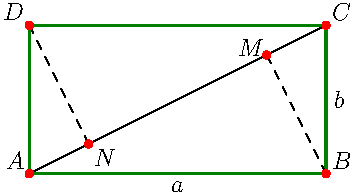
\includegraphics{Egp13_1.pdf}
  \caption{Exercice \arabic{enumi}}
  \label{fig:Egp13_1}
\end{figure}

\begin{tiny}(gp13)\end{tiny} Soit $A$, $B$, $C$, $D$  un rectangle dont les longueurs des côtés sont $a$ et $b$. On projette les points $B$ et $D$ en $M$ et $N$ sur la diagonale $(AC)$. (voir figure \ref{fig:Egp13_1}).\newline
Exprimer la longueur $MN$ en fonction de $a$ et $b$.
 
  \item \begin{tiny}(Egp14)\end{tiny} Cercles tangents à deux droites.
\begin{enumerate}
 \item On se donne deux droites $\mathcal{D}_1$, $\mathcal{D}_2$ et un point $A$. Soit $I$ un point quelconque. Caractériser par deux égalités la propriétés\newline
\og $I$ est le centre d'un cercle qui passe par $A$ et tangent à $\mathcal{D}_1$ et $\mathcal{D}_2$ \fg
\item Un repère orthonormé étant fixé, déterminer l'ensemble des centres des cercles passant par $A$ de coordonnées $(1,0)$ et tangents à deux droites orthogonales passant par l'origine du repère.  
\end{enumerate}
 
  \item \begin{figure}[ht]
 \centering
\input{Egp15_1.pdf_t}
\caption{Exercice \arabic{enumi}}
\label{fig:Egp15_1}
\end{figure}
\begin{tiny}(gp15)\end{tiny}
Dans un plan muni d'un repère, on se donne trois points $I$, $A$, $B$ respectivement de coordonnées $(1,1)$, $(1,0)$, $(0,1)$. Soit $\mathcal C$ le cercle de centre $I$ et de rayon $1$, soit $M$ un point de $\mathcal C$. La tangente en $M$ à $\mathcal C$ coupe l'axe $Ox$ en $P$ et l'axe $Oy$ en $Q$. (voir figure \ref{fig:Egp15_1})
\begin{enumerate}
 \item En utilisant la règle du dédoublement pour obtenir l'équation d'une tangente, donner des expressions simples de
\begin{displaymath}
(x(P)-1)(x(M)-1) \text{ et }(y(Q)-1)(y(M)-1) 
\end{displaymath}
en fonction de $x(M)$ et de $y(M)$.
 \item Former les équations des droites $(PB)$, $(QA)$, $(OM)$.
 \item Montrer que les droites $(PB)$, $(QA)$, $(OM)$ sont parallèles ou concourantes.
\end{enumerate}
 
  \item \begin{tiny}(Egp16)\end{tiny} Puissance d'un point par rapport à un cercle. Axe radical de deux cercles.\newline
On note $x$ et $y$ les fonctions coordonnées dans un repère orthonormal fixé. Soit $\mathcal{C}$ un cercle, il existe des réels $a$, $b$, $c$ tels que, pour tout point $M$,
\begin{displaymath}
 M \in \mathcal{C}
\Leftrightarrow p_{\mathcal{C}}(M)=0
\text{ avec }
p_{\mathcal{C}} = x^2 + y^2 +ax+by+c
\end{displaymath}
\begin{enumerate}
 \item Soit $M$ un point et $\mathcal{D}$ une droite passant par $M$ et coupant $\mathcal{C}$ en deux points $P$ et $Q$ (évenuellement confondus). Montrer que
\begin{displaymath}
 p_{\mathcal{C}}(M) = (\overrightarrow{MP}/\overrightarrow{MQ})
\end{displaymath}
\item Soit $\mathcal{C}'$ un autre cercle avec
\begin{displaymath}
p_{\mathcal{C}'} = x^2 + y^2 +a'x+b'y+c'
\end{displaymath}
Montrer que l'ensemble des points $M$ tels que 
\begin{displaymath}
 p_{\mathcal{C}}(M) = p_{\mathcal{C}'}(M)
\end{displaymath}
est une droite (axe radical des deux cercles). Montrer que l'axe radical est orthogonal à la droite des centres.
\item On se donne un cercle $\mathcal{C}$ et deux points $A$ et $B$ qui ne sont pas sur $\mathcal{C}$. \`A toute droite $\mathcal{D}$ passant par $A$ et coupant $\mathcal{C}$ en $M$ et $N$, on associe le cercle passant par $M$, $N$, $B$. Il est noté $\mathcal{C}(\mathcal{D})$. Montrer que tous les $\mathcal{C}(\mathcal{D})$ passent par un même point (autre que $B$).
\item On se donne trois cercles et les trois axes radicaux de ces cercles pris deux à deux. Montrer que ces trois droites sont parallèles ou concourantes.
\end{enumerate}

  
\end{enumerate} 
\clearpage 
\chead{géométrie plane élémentaire: corrigés.}
\begin{enumerate}
  \item \begin{tiny}(Egp01)\end{tiny} Soit $(x,y)$ les coordonnées de $M$ et $P$ le projeté cherché. Il est de la forme
\begin{displaymath}
  P = M + \lambda u
\end{displaymath}
où $u$ orthogonal $\mathcal{D}$ est de coordonnées $(2,-1)$ avec $\lambda$ tel que $P \in \mathcal{D}$:
\begin{displaymath}
  2(x+2\lambda) - (y-\lambda) + 1 = 0
  \Rightarrow
  \lambda = -\frac{2x-y+1}{5}
\end{displaymath}
On en déduit les coordonnées de $P$: 
\begin{displaymath}
(x - \frac{2}{5}(2x-y+1), y + \frac{1}{5}(2x-y+1)) 
\end{displaymath}
puis celles du symétrique $S = M + 2\lambda u$:
\begin{displaymath}
(x - \frac{4}{5}(2x-y+1), y + \frac{2}{5}(2x-y+1)).  
\end{displaymath}
 
  \item Cgp02.tex manque. 
  \item Cgp03.tex manque. 
  \item Cgp04.tex manque. 
  \item Cgp05.tex manque. 
  \item Cgp06.tex manque. 
  \item Cgp07.tex manque. 
  \item Cgp08.tex manque. 
  \item Cgp09.tex manque. 
  \item Les formules sont rassemblées en plusieurs groupes selon l'idée principale de la démonstration.\\
\begin{figure}[h!t]
 \centering
 \input{./Cgp10_1.pdf_t}
 \caption{exercice \arabic{enumi} : expressions de $R$}
 \label{fig:Cgp10_1}
\end{figure}

Le premier groupe de formules vient du théorème de l'angle au centre dans le cercle circonscrit. La figure \ref{fig:Cgp10_1} permet d'écrire $R\sin \widehat C = \frac{c}{2}$. On obtient les autres relations par des considérations analogues. La dernière s'obtient en ajoutant les expressions obtenues pour $a$, $b$, $c$.

Pour la deuxième formule on utilise le déterminant pour exprimer l'aire et la première relation du premier groupe: 
\begin{displaymath}
 2S = \det(\overrightarrow{AB},\overrightarrow{AC}) = cb\sin \widehat A = \frac{abc}{2R}
\end{displaymath}

Les quatre formules suivantes viennent de décomposition d'aires à l'aide de triangles.
\begin{figure}[h!t]
 \centering
 \input{./Cgp10_2.pdf_t}
 \caption{exercice \arabic{enumi} : rayon du cercle inscrit}
 \label{fig:Cgp10_2}
\end{figure}
Pour le calcul du rayon $r$ du cercle inscrit, on découpe le triangle $(ABC)$ en trois triangles (figure \ref{fig:Cgp10_2}) dont on connait les bases ($a$, $b$, $c$) et hauteur ($r$). La formule se déduit de
\begin{displaymath}
 A = \frac{ar}{2}+\frac{br}{2}+\frac{cr}{2} 
\end{displaymath}
 
  \item \begin{tiny}(Cgp11)\end{tiny} 
\begin{enumerate}
  \item Comme $M'$ et $N'$ sont distincts, le vecteur $\overrightarrow{M'N'}$ est, comme $\overrightarrow{u}$, une base de la direction de $\mathcal{D}$ avec $\overline{M'N'} \neq 0$ et :
\begin{displaymath}
  \overrightarrow{M'N'} = \overline{M'N'}\, \overrightarrow{u}
  \Rightarrow
  \overrightarrow{u} = \frac{1}{\overline{M'N'}} \overrightarrow{M'N'}.
\end{displaymath}
En remplaçant dans l'expression de $\overrightarrow{MN}$:
\begin{displaymath}
  \overrightarrow{MN} = \overline{MN}\, \overrightarrow{u}
   = \frac{\overline{MN}}{\overline{M'N'}}\, \overrightarrow{M'N'}.
\end{displaymath}

  \item Expression des coordonnées
\begin{center}
\renewcommand{\arraystretch}{1.3}
\begin{tabular}{|c|c|c|}
\hline
$A$ & $B$ & $C$ \\ \hline
$(0,0)$ & $(\overline{AB},0)$ & $(0,\overline{AC})$ \\ \hline 
\end{tabular}   
\end{center}

Utilisons la première question pour exprimer les coordonnées de $\overrightarrow{k}$.
\begin{displaymath}
  \overrightarrow{BC} = \overrightarrow{AC} - \overrightarrow{AB}
  = \overline{AC}\, \overrightarrow{j} - \overline{AB}\, \overrightarrow{i}
  =\overline{BC}\, \overrightarrow{k}.
\end{displaymath}
On en déduit
\begin{displaymath}
  \overrightarrow{k} = - \frac{\overline{AB}}{\overline{BC}}\overrightarrow{i}
  +\frac{\overline{AC}}{\overline{BC}}\overrightarrow{j}.
\end{displaymath}
On remplace dans
\begin{displaymath}
  \overrightarrow{AA'} = \overrightarrow{AB} + \overrightarrow{BA'}
  = \overline{AB}\overrightarrow{i} + \overline{BA'}\overrightarrow{k}
\end{displaymath}
D'où
\begin{displaymath}
  \overrightarrow{AA'} = \left( \overline{AB} - \overline{BA'}\,\frac{\overline{AB}}{\overline{BC}}\right)\overrightarrow{i}
  + \overline{BA'}\,\frac{\overline{AC}}{\overline{BC}}\overrightarrow{j}
\end{displaymath}

\begin{center}
\renewcommand{\arraystretch}{1.5}
\begin{tabular}{|c|c|c|}
\hline
$A'$ & $B'$ & $C'$ \\ \hline
$(\overline{A'C}\,\frac{\overline{AB}}{\overline{BC}},-\overline{A'B}\,\frac{\overline{AC}}{\overline{BC}})$ 
& $(0,\overline{AB'})$ 
& $(\overline{AC'},0)$ \\ \hline 
\end{tabular} 
\end{center}
La condition d'alignement exprimée avec les coordonnées s'écrit comme la nullité du déterminant
\begin{displaymath}
  \begin{vmatrix}
    \overline{A'C} \,\overline{AB} & -\overline{A'B}\,\overline{AC} & \overline{BC} \\
    0 & \overline{AB'} & 1 \\
    \overline{AC'} & 0 & 1
  \end{vmatrix}
= 0
\end{displaymath}
Elle est équivalente à
\begin{displaymath}
  -\overline{A'C}\,\overline{B'A}\,\overline{AB}
  +\overline{A'B}\,\overline{AC}\,\overline{C'A}
  -\overline{B'A}\,\overline{C'A}\,\overline{BC} = 0
\end{displaymath}
On obtient la condition demandée en introduisant $C'$ dans $\overline{AB}$, $B'$ dans $\overline{AC}$, $A'$ dans $\overline{BC}$.\newline
La condition est indépendante des vecteurs unitaires car c'est un produit de 3 fractions. Pour chacune, le numérateur et le dénominateur sont multipliés par le même nombre lors d'un changement de vecteur unitaire.
\end{enumerate}
 
  \item Cgp12.tex manque. 
  \item \begin{tiny}(Cgp13)\end{tiny} Le projeté $N$ de $D$ est de la forme
\begin{displaymath}
  N = D +\lambda 
  \begin{pmatrix}
    b\\ -a
  \end{pmatrix}
\end{displaymath}
où $N \in (AB)$ c'est à dire que 
\begin{displaymath}
  bx_N - ay_N = 0.
\end{displaymath}
On en déduit
\begin{displaymath}
  \lambda = \frac{ab}{a^2 + b^2}, \;DN = \frac{ab}{\sqrt{a^2+b^2}}.
\end{displaymath}
La figure est symétrique par  rapport au milieu de $AB$ donc
\begin{displaymath}
  BM = DN, \; AN = CM.
\end{displaymath}
Par le théorème de Pythagore dans $AND$,
\begin{displaymath}
  AN = \frac{b^2}{\sqrt{a^2 + b^2}}.
\end{displaymath}
On en déduit
\begin{displaymath}
  MN = \sqrt{a^2 + b^2} -2 \frac{b^2}{\sqrt{a^2+b^2}}
  = \frac{a^2 - b^2}{\sqrt{a^2 + b^2}}.
\end{displaymath}



 
  \item \begin{tiny}(Cgp14)\end{tiny} Cercles tangents à deux droites.
\begin{figure}[h!t]
 \centering
 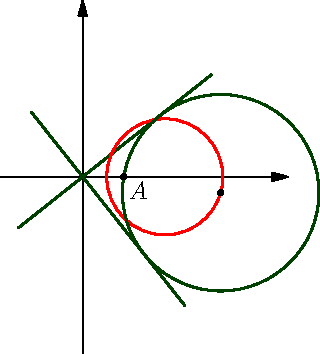
\includegraphics{./Cgp14_1.pdf}
 % Cgp14_1.pdf: 0x0 pixel, 0dpi, nanxnan cm, bb=
 \caption{Exercice \arabic{enumi} Cercles tangents à deux droites}
 \label{fig:Cgp14_1}
\end{figure}

\begin{enumerate}
 \item Le point $I$ est le centre d'un cercle tangent aux deux droites $\mathcal{D}_1$ et $\mathcal{D}_2$ si et seulement si il est à égale distance des deux droites ou encore si et seulement si il est sur une des deux bissectrices des deux droites.
 \item On se donne les deux droites par leurs vecteurs directeurs $\overrightarrow{e}_\theta$ et $\overrightarrow{e}_{\theta +\frac{\pi}{2}}$:
\begin{displaymath}
 \mathcal{D}_1(\theta)= O+\Vect(\overrightarrow{e}_\theta),\hspace{0.3cm}
 \mathcal{D}_2(\theta)= O+\Vect(\overrightarrow{e}_{\theta +\frac{\pi}{2}})
\end{displaymath}
Les centres des cercles passant par $A$ et tangents aux deux droites sont les points $C$ des bissectrices pour lesquels $AC$ est aussi la distance aux bissectrices.\newline
La distance d'un point $M$ à $\mathcal{D}_1(\theta)$ est 
\begin{displaymath}
|\det(\overrightarrow{OM},\overrightarrow{e}_\theta)| 
\end{displaymath}
Les points de la première bissectrice sont de la forme
 \begin{displaymath}
  O+\lambda \overrightarrow{e}_{\theta +\frac{\pi}{4}}
 \end{displaymath}
Soit $C$ un tel point. En notant $\varphi = \theta +\frac{\pi}{4}$, il s'agit d'une définition \emph{polaire} de $C$. La distance à $\mathcal{D}_1(\theta)$ à $C$ est $\frac{|\lambda|}{\sqrt{2}}$. Sa distance à $A$ est
\begin{displaymath}
 \sqrt{(\lambda\cos \varphi -1)^2 + (\lambda\sin(\varphi))^2}
\end{displaymath}
En élevant au carré, la condition assurant que $C$ est le centre d'un cercle vérifiant les conditions s'écrit donc
\begin{displaymath}
 \frac{\lambda^2}{2}=
(\lambda\cos \varphi -1)^2 + (\lambda\sin(\varphi))^2
\end{displaymath}
En développant et simplifiant puis en passant aux coordonnées cartésiennes, on montre que cette condition est équivalente à
\begin{displaymath}
 (x(C)-2)^2 + y(C)^2 = 2
\end{displaymath}
Le point $C$ doit donc être sur le cercle de centre le point de coordonnées $(2,0)$ et de rayon $\sqrt{2}$.\newline
Les points de la deuxième bissectrice sont de la forme
 \begin{displaymath}
  O+\lambda \overrightarrow{e}_{\theta -\frac{\pi}{4}}
 \end{displaymath}
Soit $C$ un tel point. En notant $\varphi = \theta -\frac{\pi}{4}$, il s'agit d'une définition \emph{polaire} de $C$. La suite des calculs est exactement la même exprimée avec $\varphi$. On obtient donc le même cercle, paramétré différement selon qu'il est coupé par l'une ou l'autre des bissectrices.
\end{enumerate} 
  \item Cgp15.tex manque. 
  \item Cgp16.tex manque. 
\end{enumerate} 
\end{document}